\section{Benchmark Protocol}
\label{sec:benchmarks}

This section reports a minimal synthetic accounting benchmark. These are not quantum-circuit simulations and are not hardware experiments. They only validate the bookkeeping behavior of \(\Lambda_{\mathrm{glob}}\), \(\Lammsg\), dense-width proxies, and SLMS exponent proxies on generated tree/resource instances.

\subsection{Synthetic accounting benchmarks}

The first benchmark layer is purely combinatorial. It generates rooted trees, assigns local costs \(\xi_b\), local norm factors \(\kappa_b\), width proxies, and local marginalizability flags, then computes:
\[
\Lambda_{\mathrm{glob}},\qquad
\max_b\log\xi_b,\qquad
\Lambda_{\mathrm{path}},\qquad
\Lambda_{\mathrm{subtree}},\qquad
\Lammsg,\qquad
\weff+2\Lammsg .
\]
This validates the behavior of the burden definitions before any quantum-circuit backend is implemented.

The accounting implementation consists of:
\begin{itemize}[leftmargin=1.2cm]
\item \texttt{benchmarks/generate\_tree\_resource\_network.py}, which generates balanced binary trees, chains, star-like trees, and random grammar-like trees with controlled resource placement modes;
\item \texttt{benchmarks/compute\_synthetic\_burdens.py}, which computes global, bag, path, subtree, and recurrence-based message burdens from the generated CSV file;
\item \texttt{benchmarks/certify\_synthetic\_lm.py}, which applies a conservative synthetic local-marginalizability certificate and generates active-child sets.
\item \texttt{benchmarks/run\_examples.sh} and \texttt{benchmarks/plot\_burdens.py}, which generate the synthetic examples below, write \texttt{benchmarks/results/summary.csv}, and produce two dependency-free SVG plots.
\end{itemize}

\subsection{Synthetic accounting outputs}

Running \texttt{benchmarks/run\_examples.sh} produces the following accounting table. Values are natural-log cost proxies. The column \(\weff+2\Lammsg\) is the scalar-sampling exponent proxy appearing in the SLMS bound, while \(\wTN\) is the dense-width column. As of the 2026-04-26 baseline-implementation pass, \(\wTN\) is computed from the underlying graph via NetworkX's \texttt{treewidth\_min\_fill\_in} heuristic (column \texttt{w\_tn\_source = computed} in the per-row CSVs); earlier revisions used a hand-set proxy.

\begin{center}
\small
\begin{tabular}{lrrrrr}
\toprule
Case & Resources & \(\Lambda_{\mathrm{glob}}\) & \(\Lammsg\) & \(\wTN\) computed & \(\weff+2\Lammsg\) \\
\midrule
balanced leaf-local & 32 & 8.396 & 0.262 & 1.000 & 1.525 \\
balanced path-active & 37 & 9.707 & 1.574 & 1.000 & 4.148 \\
uniform chain & 40 & 10.495 & 10.495 & 1.000 & 21.989 \\
clustered subtree & 31 & 8.133 & 8.133 & 1.000 & 18.267 \\
grid accounting & 9 & 2.361 & 0.262 & 11.000 & 1.525 \\
\bottomrule
\end{tabular}
\end{center}

All five rows now report computed treewidth: balanced trees and the chain give \(\wTN=1\) as expected, and the grid case (an honest \(9\times 9\) grid graph; see \texttt{generate\_tree\_resource\_network.py --shape grid}) gives \(\wTN=11\) under \texttt{treewidth\_min\_fill\_in} (an upper-bound heuristic; the optimal value for the \(9\times 9\) grid is \(9\)). The first two rows reproduce the global-magic accounting separations: global burden scales with the number of resource leaves, while \(\Lammsg\) is constant or path-like. The chain and clustered rows are negative controls where the active-child recurrence does not improve the magic burden. The final row is an accounting analogue of Proposition~\ref{thm:dense-width-separation}: the dense-width column is large while the effective-width-plus-message column is small. The generated plots are stored in \texttt{benchmarks/results/} as \texttt{burdens\_global\_vs\_msg.svg} and \texttt{burdens\_dense\_vs\_slms.svg}.

\subsection{Implemented and conceptual comparator diagnostics}

The repository separates implemented exponent proxies from conceptual competitors. The focused-width proxy row is a legacy resource-separator diagnostic. The Codsi--Laakkonen, pyzx, and STN-style rows below are implemented comparator diagnostics with the limitations stated in the table; they are not dominance claims and not faithful implementations of every published simulator in the corresponding family.

\begin{center}
\scriptsize
\resizebox{\linewidth}{!}{%
\begin{tabular}{llllll}
\toprule
Method & Implemented here? & Parameter & Output file & Limitation & Relation to SLMS \\
\midrule
Dense TN proxy & yes & \(\wTN\) proxy & \texttt{results/baseline\_results.csv} & graph-width proxy, no tensor timings & dense contraction comparator \\
Global PWB proxy & yes & \(2\Lambda_{\mathrm{glob}}\) & \texttt{results/baseline\_results.csv} & global quasiprobability burden only & charges all resource labels globally \\
Naive hybrid proxy & yes & \(\weff+2\Lambda_{\mathrm{glob}}\) & \texttt{results/baseline\_results.csv} & no local marginalization & same \(\weff\), global magic burden \\
SLMS proxy & yes & \(\weff+2\Lammsg\) & \texttt{results/baseline\_results.csv} & certificate exponent, not runtime & proposed certified parameter \\
Focused-width proxy & yes & active resource separator score & \texttt{results/baseline\_results.csv} & not exact focused tree-width & sanity comparator only \\
Focused tw/rw diagnostic & yes & focused tw/rw upper bound & \texttt{results/baseline\_results.csv} & exact only for small cases & Codsi--Laakkonen comparator \\
pyzx + BG proxy & yes & reduced \(T\)-count exponent & \texttt{results/baseline\_results.csv} & synthetic encoding; no ZX cutting & ZX-inspired comparator \\
pyzx partition heuristic & yes & partitioned reduced \(T\)-count & \texttt{results/baseline\_results.csv} & heuristic; not Sutcliffe--Kissinger & ZX partition diagnostic \\
STN-style proxy & yes & tableau + BG upper bound & \texttt{results/baseline\_results.csv} & not Masot-Llima/Nakhl STN & stabilizer-TN-inspired comparator \\
ZX partitioning & no & not computed & \texttt{results/baseline\_results.csv} & no Sutcliffe--Kissinger backend & discussion-only competitor \\
STN / MAST exact & no & not computed & \texttt{results/baseline\_results.csv} & no exact STN/MAST backend & discussion-only competitor \\
\bottomrule
\end{tabular}
}
\end{center}

\subsection{Certificate evidence on lambeq reader and fallback structured instances}

The directory \texttt{experiments/slms\_certificate/} contains a second reproducibility layer. In the present run, a clean Python 3.11 environment was created under \texttt{/tmp/slms\_lambeq\_py311}. In that environment, lambeq 0.5.0 imported successfully and exposed Bobcat, DepCCG, CCG, and Web parser classes. None of the three CCG-grammatical parser paths produced parsed diagrams in the run environment, due to upstream issues that are not specific to this artifact:
\begin{itemize}[leftmargin=1.2cm]
\sloppy
\item \texttt{BobcatParser} fetches its model from the URL \url{https://qnlp.cambridgequantum.com/models/bobcat/latest/version.txt} hardcoded in lambeq 0.5.0's \path{model_downloader.py}. In the audited run, model retrieval failed before parser construction completed, with the exact exception recorded in \path{results/real\_lambeq\_parse\_log.txt} and the blocker reports.
\item \texttt{DepCCGParser} requires the external \texttt{depccg} package. In the audited run, \texttt{pip install depccg} failed while getting wheel requirements because the build requested Cython and NumPy before building extension modules; importing \texttt{DepCCGParser} then failed with \texttt{ModuleNotFoundError: No module named 'depccg'}. The lambeq 0.5.0 documentation also notes that DepCCG-related functionality is no longer actively supported.
\item \texttt{WebParser} failed against the lambeq web service in the executed environment; the exact exception is recorded in \path{results/real_lambeq_parse_log.txt} and \path{results/qnlp\_extraction\_probe.json}.
\end{itemize}
The pipeline therefore fell back to lambeq's local \texttt{cups\_reader}, which produced 120 lambeq LinearReader diagrams. These are real lambeq-generated diagrams but not CCG-parsed outputs; the linear cup/cap structures contain no non-Clifford resource annotations, so they are useful as an end-to-end lambeq import/diagram/graph-extraction check but not as nontrivial QNLP resource evidence.

For the nontrivial certificate experiment, the artifact then used fallback structured instances. These are lambeq-compatible grammar-tree and stabilizer-compressed accounting instances, not parser-generated lambeq outputs. The manifest records fallback-plus-reader mode: fallback data is the primary certificate evidence, and the lambeq reader data is a sidecar extraction check. The generated files are:
\begin{itemize}[leftmargin=1.2cm]
\item \texttt{results/environment\_report.json} and \texttt{results/environment\_report.txt};
\item \texttt{results/real\_lambeq\_parse\_log.txt} and \texttt{results/real\_lambeq\_instances.json};
\item \texttt{results/qnlp\_extraction\_probe.json} and \texttt{results/qnlp\_extraction\_probe.md};
\item \texttt{results/end\_to\_end\_slms\_wallclock.*};
\item \texttt{results/lambeq\_reader\_certificate\_results.csv};
\item \texttt{results/lambeq\_reader\_baseline\_results.csv};
\item \texttt{results/lambeq\_reader\_dense\_contraction\_baseline.csv};
\item \texttt{results/fallback\_instances.json};
\item \texttt{results/slms\_certificate\_results.csv};
\item \texttt{results/slms\_certificate\_summary.json};
\item \texttt{results/slms\_certificate\_failures.csv};
\item \texttt{results/baseline\_results.csv};
\item \texttt{results/dense\_contraction\_baseline.csv};
\item \texttt{results/slms\_scalar\_estimator\_results.csv};
\item \texttt{results/worked\_certificate\_recurrence.csv};
\item diagnostic plots under \texttt{figures/}.
\end{itemize}

These experiments are certificate-evidence experiments, not wall-clock simulator benchmarks. They test whether the SLMS certificate is non-vacuous on structured instances and how its exponent proxy compares to dense-width and global-magic proxies.

\paragraph{Hard-blocker ledger summary.}
The artifact includes a machine-checkable and human-readable blocker ledger. Parser-generated lambeq/QDisCoCirc resource instances, end-to-end SLMS wall-clock benchmarking on such instances, exact Sutcliffe--Kissinger ZX cutting or \(k\)-partitioning, exact Masot-Llima/Nakhl STN or MAST baselines, and a worked certificate from a parser-generated lambeq resource instance are all marked \emph{blocked}. Public DOI release is marked \emph{partially mitigated}: the local artifact is prepared, but the DOI placeholder must not be replaced until Zenodo mints an archive. The fallback certificate artifact itself is resolved as executable evidence for the recurrence mechanics, not as parser-level QNLP coverage.

\begin{center}
\small
\begin{tabular}{lr}
\toprule
Quantity & Value from executed run \\
\midrule
Primary certificate instances & 120 \\
Lambeq LinearReader graph-only instances & 120 \\
Fallback instances & 120 \\
Parser-generated lambeq instances & 0 \\
Mode used & \texttt{fallback\_with\_lambeq\_reader\_evidence} \\
Certificate passes/failures & 105/15 \\
Certificate pass rate & 87.5\% \\
Median \(\Lammsg\) & 0.924 \\
Range of \(\Lammsg\) & 0.262--8.396 \\
Median \(\weff\) proxy & 1.000 \\
Range of \(\weff\) proxy & 1.000--5.000 \\
Range of dense \(\wTN\) proxy & 1.000--10.000 \\
Median SLMS exponent proxy \(\weff+2\Lammsg\) & 3.574 \\
Median global PWB proxy \(2\Lambda_{\mathrm{glob}}\) & 8.396 \\
\bottomrule
\end{tabular}
\end{center}

The lambeq reader sidecar has 120 graph-only instances, 120/0 certificate passes/failures, \(\Lammsg=0\), \(\Lambda_{\mathrm{glob}}=0\), and \(\weff+2\Lammsg=1\) for every instance. These values are expected because the local reader diagrams do not provide non-Clifford resource placements. We therefore do not use the reader sidecar as evidence for the separator-local magic reduction; it only verifies that the artifact can import lambeq, generate diagrams locally, extract graphs, and run the certificate machinery on those graphs. Figure~\ref{fig:certificate-evidence} plots \(\Lammsg\) against \(\Lambda_{\mathrm{glob}}\) and the per-method exponent comparison; Figure~\ref{fig:certificate-pass} shows the \(\Lammsg\) histogram and pass/fail counts.

\begin{figure}[t]
\centering
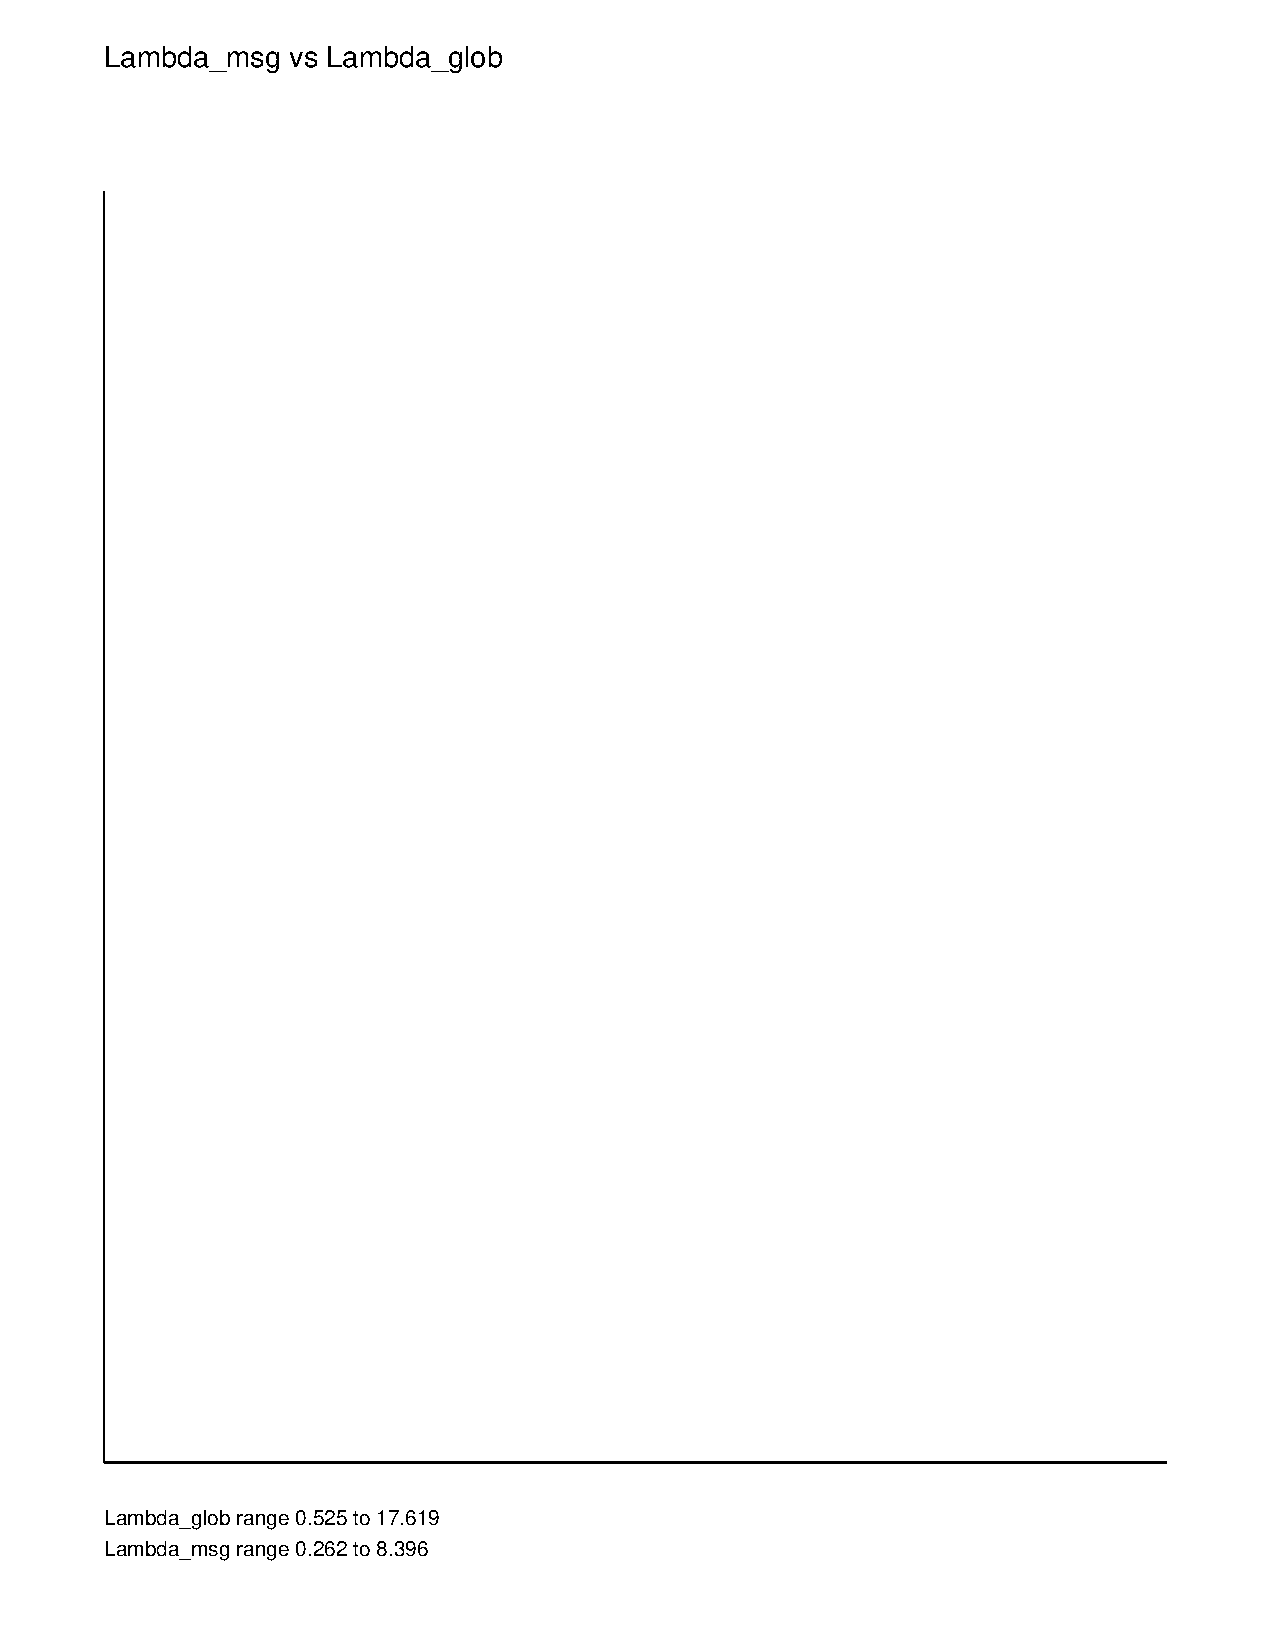
\includegraphics[width=0.46\linewidth]{figures/exp_lambda_msg_vs_lambda_glob.pdf}
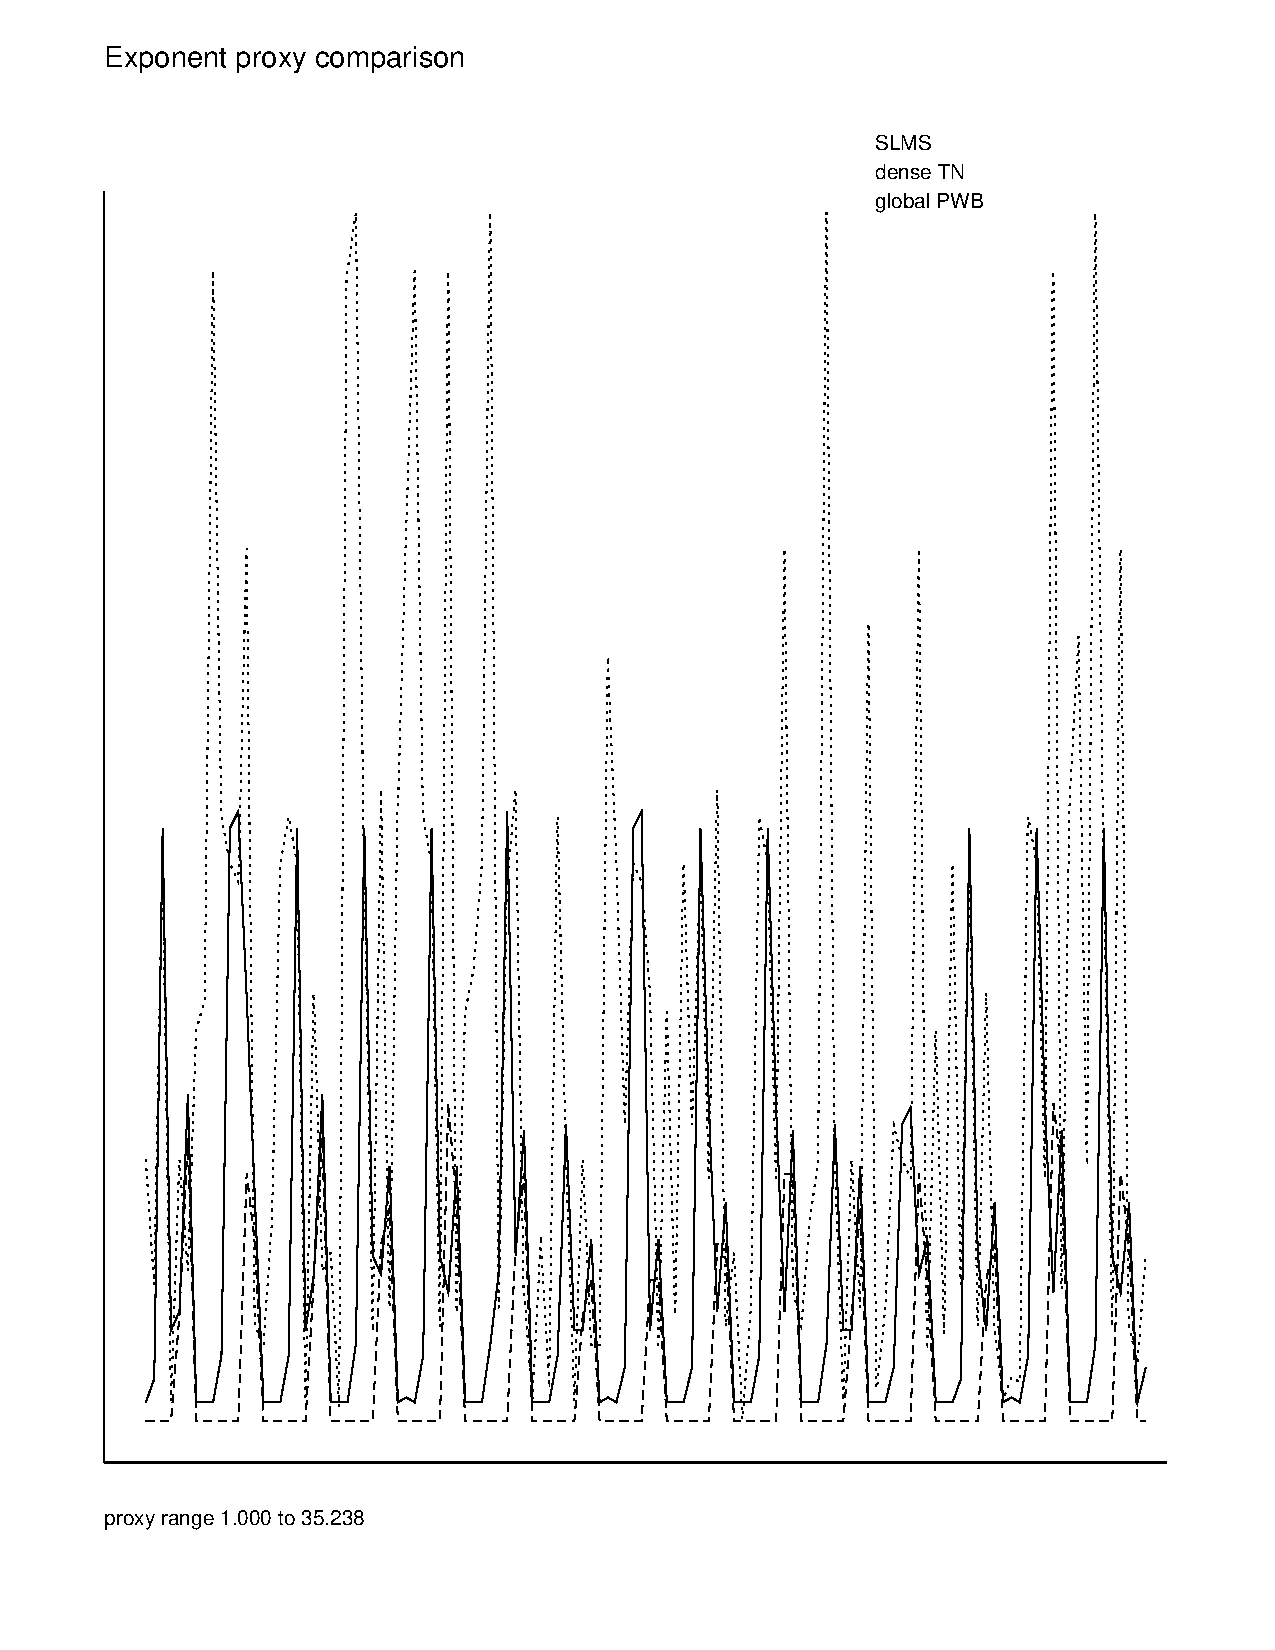
\includegraphics[width=0.46\linewidth]{figures/exp_exponent_proxy_comparison.pdf}
\caption{Fallback certificate-evidence diagnostics. Left: \(\Lammsg\) versus \(\Lambda_{\mathrm{glob}}\). Right: exponent proxy comparison across the generated structured instances. These plots are generated artifacts, but they are not runtime measurements and not parser-generated lambeq data.}
\label{fig:certificate-evidence}
\end{figure}

\begin{figure}[t]
\centering
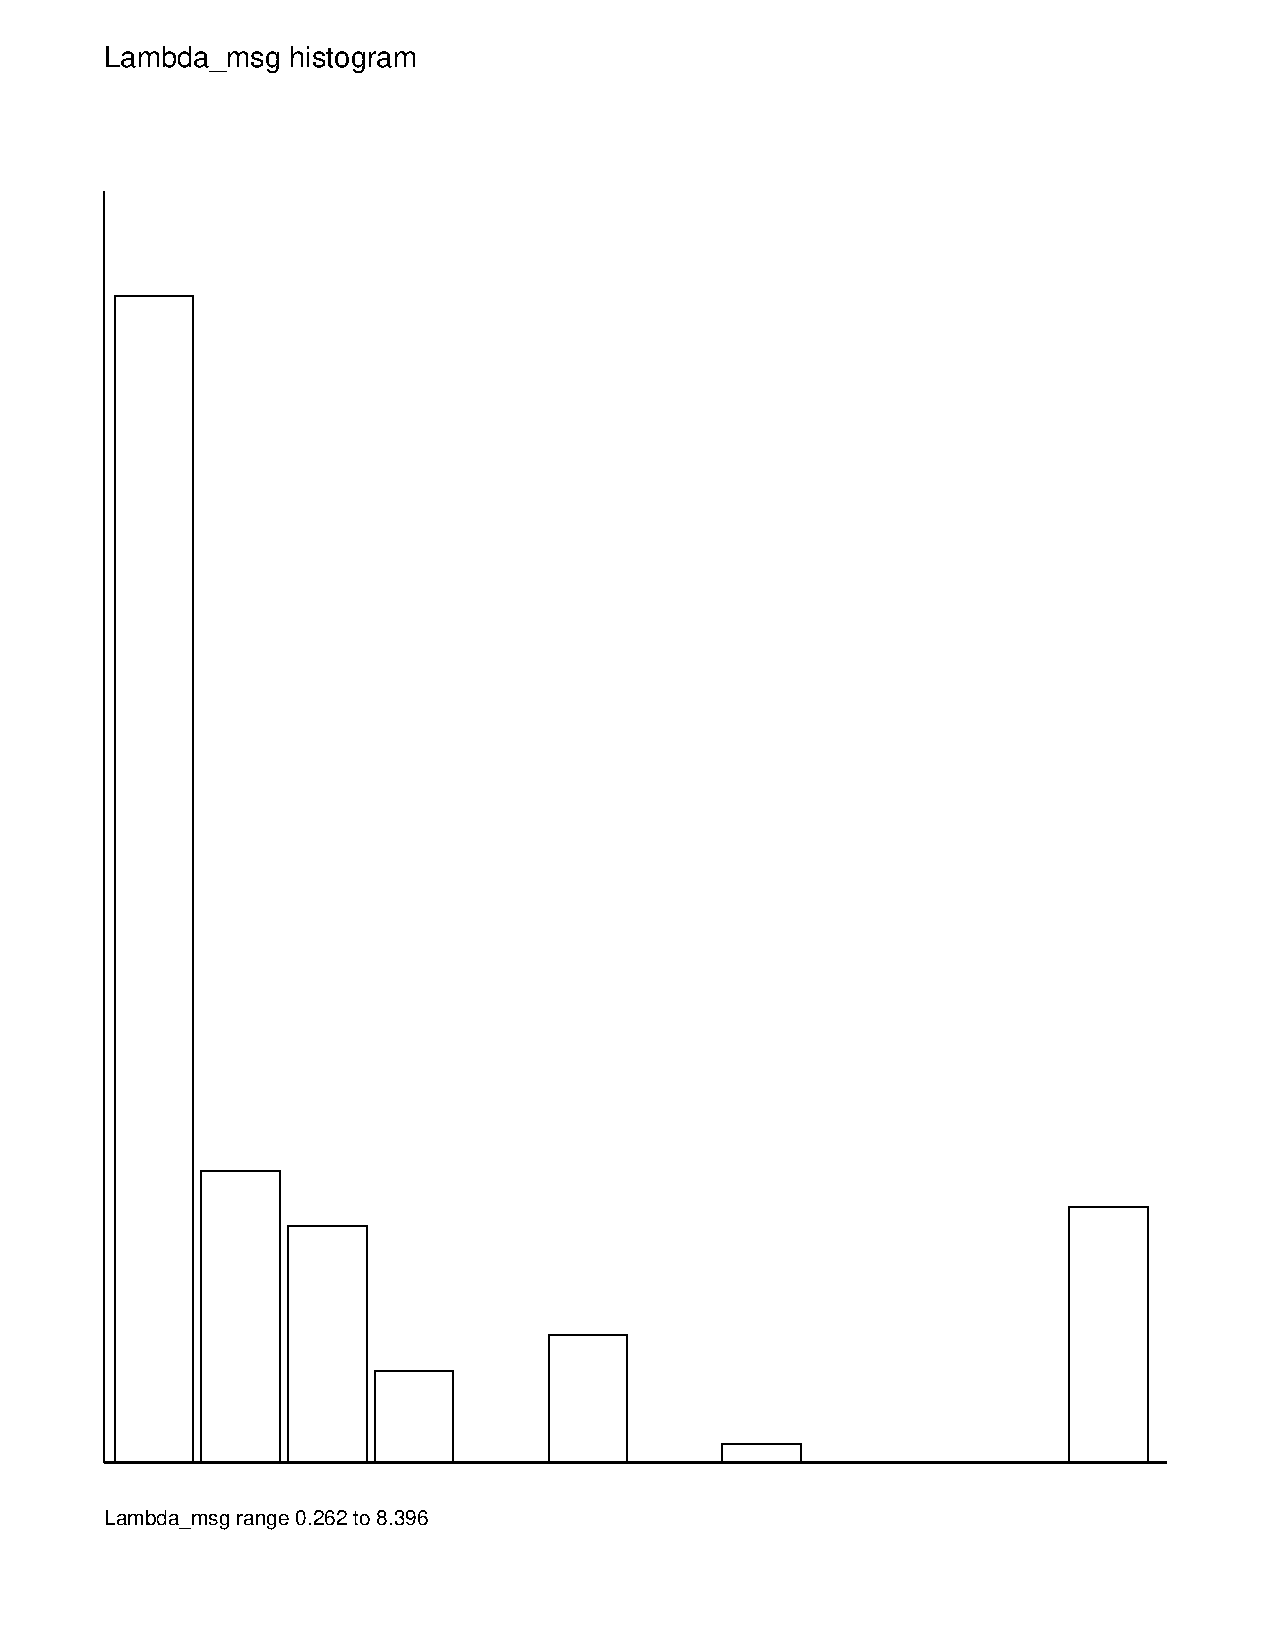
\includegraphics[width=0.46\linewidth]{figures/exp_lambda_msg_histogram.pdf}
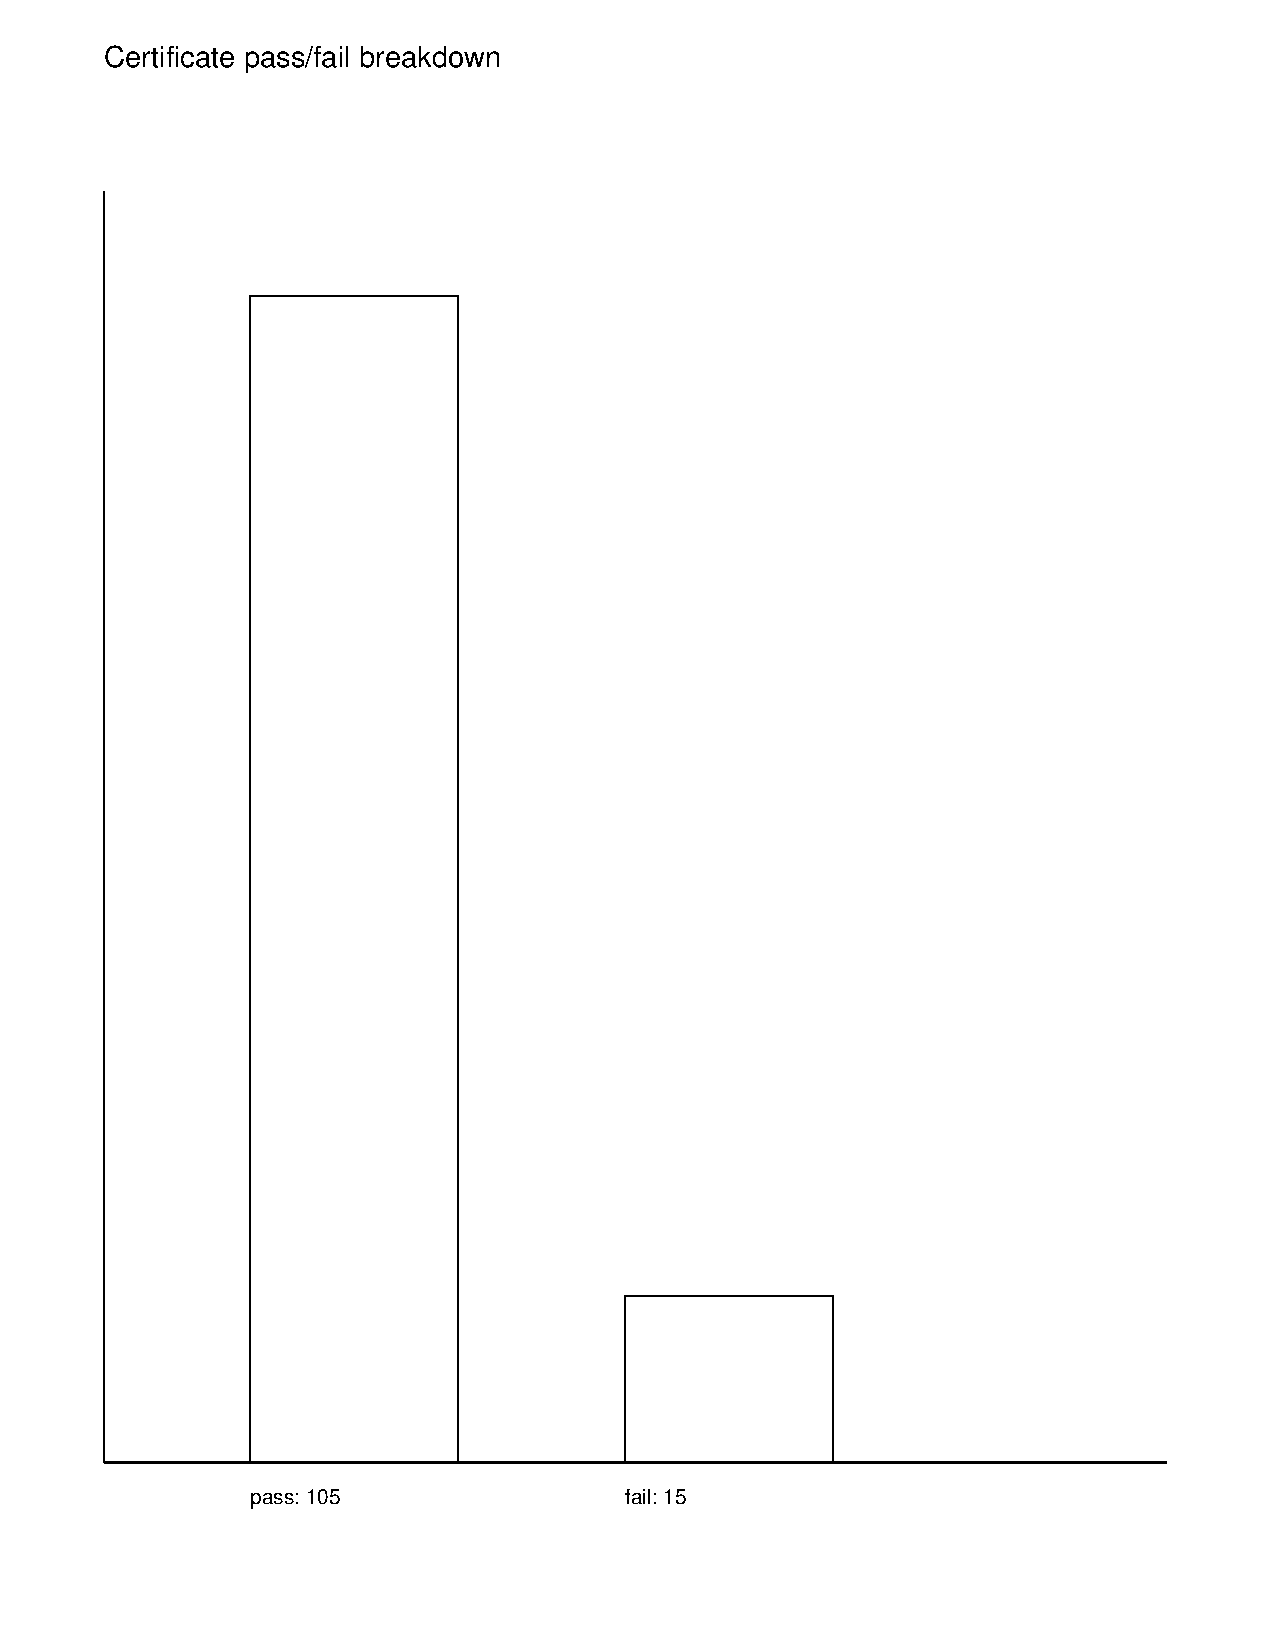
\includegraphics[width=0.46\linewidth]{figures/exp_certificate_pass_rate.pdf}
\caption{Fallback certificate distribution and pass/fail counts. The failure count is intentional: the fallback generator includes negative controls where local marginalization certificates are missing.}
\label{fig:certificate-pass}
\end{figure}

\subsection{Comparison baselines: focused width, ZX, and STN-style upper bounds}
\label{sec:bench-comparators}

The artifact's \texttt{baselines.py} now computes per-instance numerical exponents for three additional comparators. None of them is claimed to dominate SLMS; the purpose is to give an honest empirical reading of where the SLMS exponent sits relative to recent literature.

\paragraph{Codsi--Laakkonen focused tree-width and focused rank-width.}
Implemented exactly via balanced-separator enumeration for instances with \(\le 22\) vertices, with a heuristic upper bound otherwise. Focused rank-width is computed by recursive bipartition of the special set \(S\) (the set of resource bags) with cut-rank evaluated over \(\mathbb F_2\); this is exact for small special sets and an upper-bound diagnostic otherwise. We report the natural-log Codsi--Laakkonen runtime exponent \((\log_{3/2} 4)\cdot\mathrm{frw}_S\cdot\log|S|\) per Theorem~8 of Codsi and Laakkonen~\citep{CodsiLaakkonen2026}, using the implemented focused-rank-width value. Across the 120 fallback instances: median focused tree-width diagnostic is \(4\) (range \(1\)--\(63\)); median focused rank-width diagnostic is \(3\) (range \(1\)--\(25\)); median Codsi--Laakkonen exponent diagnostic is \(37.92\) (range \(2.37\)--\(347.44\)).

\paragraph{ZX-inspired diagnostic (pyzx \texttt{full\_reduce} + Bravyi--Gosset stabilizer rank).}
For each instance we build a synthetic Clifford+\(T\) circuit on \(|V|\) qubits in which a \(T\) gate is placed on the qubit at every resource bag and a \(CZ\) is placed on every parent--child edge (with \(H\) layers at the boundary). We run \(\mathtt{pyzx.simplify.full\_reduce}\) and report \(\alpha_{\mathrm{BG}}\cdot T_{\mathrm{reduced}}\cdot\ln 2\) with \(\alpha_{\mathrm{BG}}=0.396\) \citep{BravyiGosset2016}. This synthetic encoding is consistent across instances but is not the original quantum circuit. Across the 120 fallback instances: median \(T_{\mathrm{reduced}}=16\) (range \(2\)--\(69\)); median ZX exponent is \(4.39\) (range \(0.55\)--\(18.94\)). The artifact also reports a pyzx graph \(k\)-partition heuristic after \(\mathtt{full\_reduce}\), minimizing a conservative partition score \(\max_j \alpha_{\mathrm{BG}}T_j\ln2 + |\partial|\,\ln2+\ln k\) for \(k\le4\). This is a reproducible partition diagnostic, not the Sutcliffe--Kissinger algorithm. \(\mathtt{pyzx.simplify.full\_reduce}\) and this heuristic do not invoke ZX cutting or parametric rewriting; the Sutcliffe--Kissinger \(k\)-partitioning and parametric-rewriting algorithms \citep{Sutcliffe2024KPartition,SutcliffeKissinger2024Cutting,SutcliffeKissinger2025Parametric} are stronger comparators that we do not implement here.

\paragraph{Stabilizer-tensor-network proxy.}
The exact Masot-Llima--Garc\'ia-S\'aez \citep{MasotLlimaGarciaSaez2024} and Nakhl et al.\ \citep{NakhlEtAl2025} algorithms are not implemented in this artifact. We report a tableau-plus-Bravyi--Gosset upper-bound proxy \(\alpha_{\mathrm{BG}}\cdot T+\log\max(1,n_{\mathrm{active\,resource}})\) (natural log) for our synthetic Clifford+\(T\) encoding. Across the 120 instances: median STN-style proxy exponent is \(8.01\) (range \(0.55\)--\(23.30\)). This is not a faithful reimplementation of the published algorithms and not a lower bound on stabilizer-tensor-network simulation; it is an upper-bound comparator only.

\paragraph{Empirical SLMS comparison.}
For each fallback instance, the SLMS exponent \(\weff+2\Lammsg\) (median \(3.57\), range \(1.52\)--\(18.27\)) is compared against the implemented diagnostics on the same instance. Counts where the SLMS exponent is strictly smaller than the comparator diagnostic are: \(101/120\) versus the implemented Codsi--Laakkonen Theorem 8 exponent diagnostic; \(66/120\) versus the pyzx \texttt{full\_reduce}+Bravyi--Gosset diagnostic; \(66/120\) versus the pyzx \(k\)-partition heuristic; and \(69/120\) versus the STN-style upper-bound proxy. These ratios are exponent-bound comparisons on a fixed synthetic encoding and a single fallback corpus; they are not wall-clock simulator comparisons or proofs of separation. A small SLMS exponent on a particular instance is evidence that this certificate identifies an easy regime, not evidence that competing simulators fail.

\paragraph{Wall-clock timings.}
The artifact records per-instance wall-clock seconds for each new comparator. Median wall-clock cost across the 120 instances: focused tree-width and focused rank-width together \(0.12\,\mathrm{s}\) (max \(0.91\,\mathrm{s}\)), pyzx \texttt{full\_reduce} \(5.8\times 10^{-3}\,\mathrm{s}\) (max \(0.04\,\mathrm{s}\)), pyzx partition heuristic \(7.9\times10^{-3}\,\mathrm{s}\) (max \(0.05\,\mathrm{s}\)), and STN-style proxy \(<10^{-4}\,\mathrm{s}\). The lambeq LinearReader sidecar instances also receive these computations but produce zeros because the reader output carries no non-Clifford resource annotations. Figure~\ref{fig:focused-proxy} compares the legacy focused-width proxy against the SLMS exponent.

\subsection{Executed dense contraction and scalar-estimator microbenchmarks}

To separate proxy accounting from executed code, the artifact also runs two small implementation checks. First, \texttt{dense\_contraction\_baseline.py} builds numeric bond-dimension-2 tensor networks from small graph instances and contracts them with \texttt{opt\_einsum}. This is a real dense contraction baseline for generated tensor data, but only on small graph-derived instances; it is not a real lambeq circuit benchmark. In the current run, 24 fallback-derived instances were contracted. The median optimized FLOP estimate was \(212\), the median largest intermediate size was \(8\), and the median contraction time was approximately \(2.2\times 10^{-4}\) seconds. The largest optimized FLOP estimate in this small run was \(176256\), with largest intermediate size \(4096\). A second sidecar dense contraction run on 24 lambeq LinearReader graphs had median optimized FLOP estimate \(124\), median largest intermediate size \(4\), and median contraction time approximately \(1.7\times 10^{-4}\) seconds.

Second, the scalar-estimator script runs a certificate-controlled signed-sampling microbenchmark on 32 passing fallback certificates, with 20000 samples per instance. This tests the sampling dependence and records empirical variance and runtime, but it is not a QNLP simulator. The median absolute error from the synthetic target value \(1\) was \(5.02\times 10^{-3}\), and the median standard error was \(6.66\times 10^{-3}\). These values are reported in the scalar-estimator CSV under \texttt{results/}.

\begin{figure}[t]
\centering
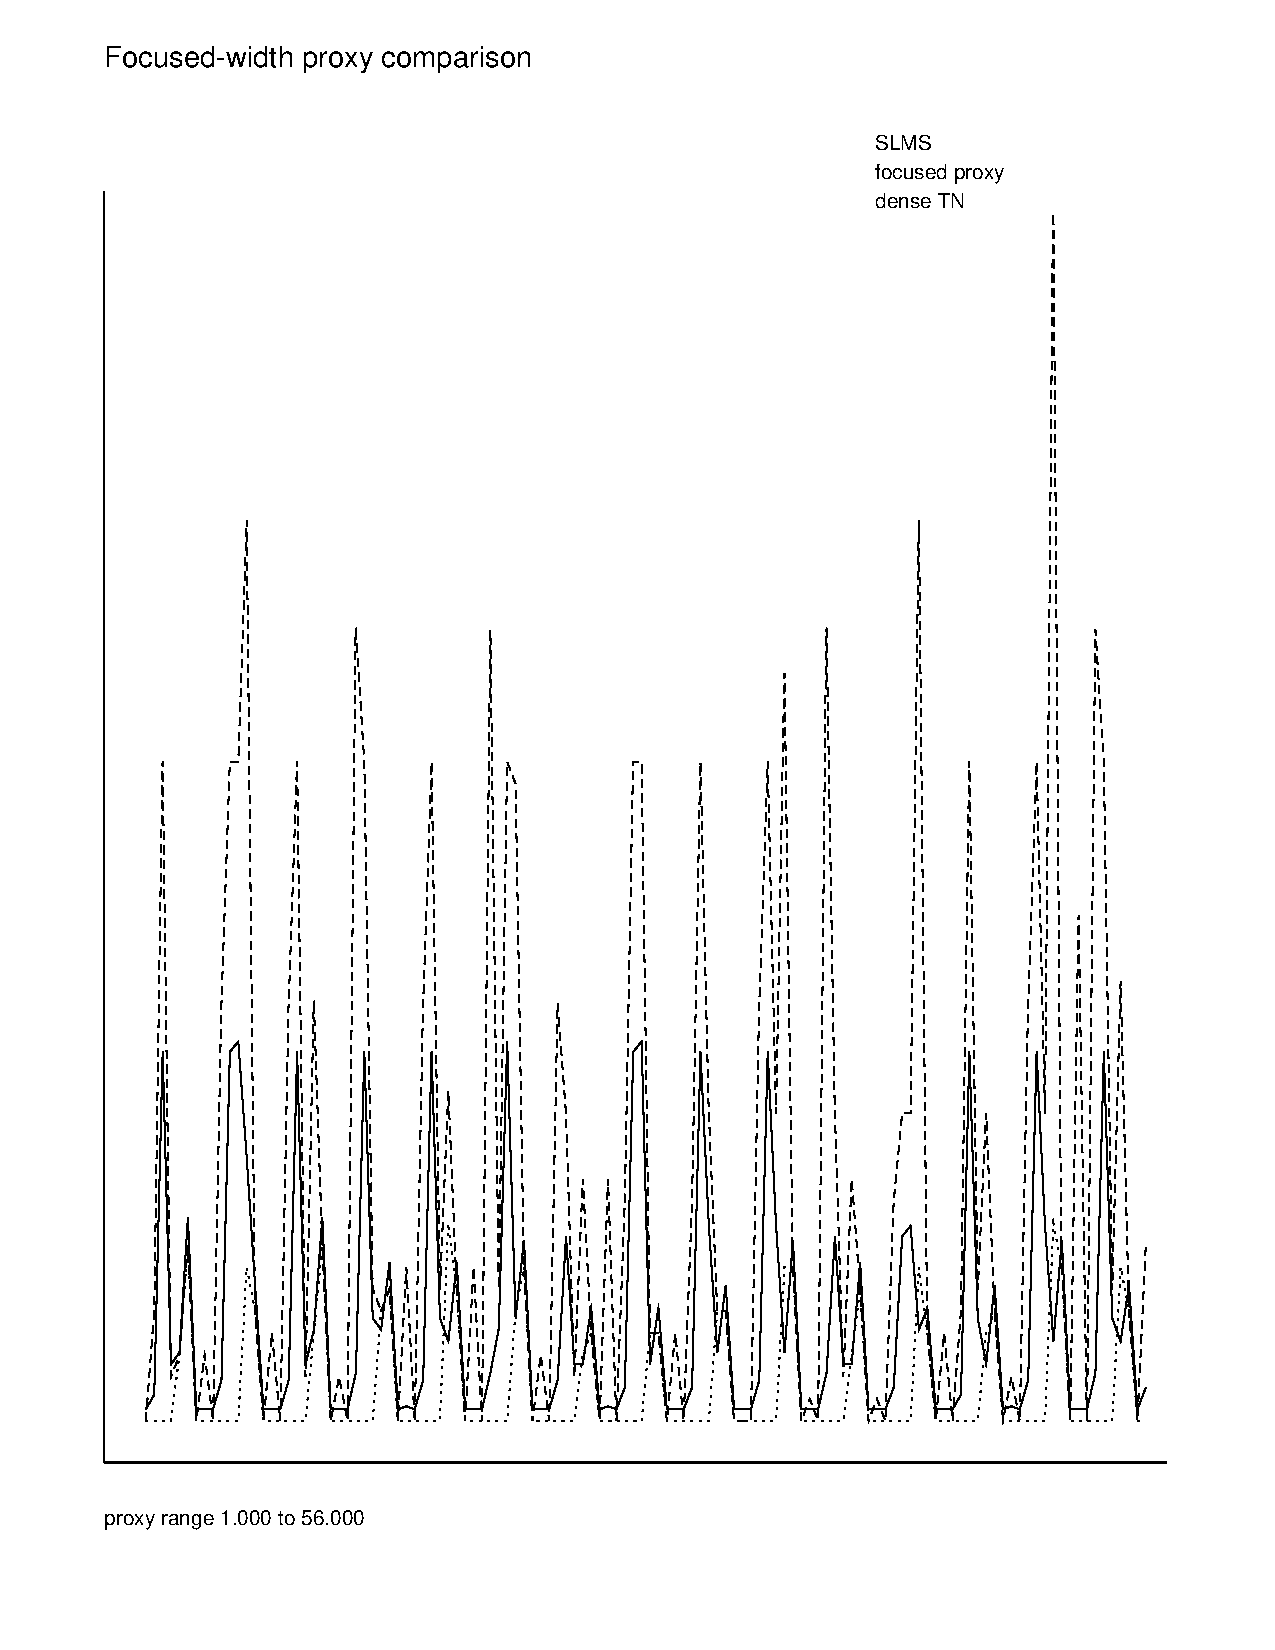
\includegraphics[width=0.48\linewidth]{figures/exp_focused_width_proxy_comparison.pdf}
\caption{Comparison with the implemented focused-width proxy. The plotted quantity is a resource-weighted separator proxy, not exact focused tree-width or focused rank-width.}
\label{fig:focused-proxy}
\end{figure}

\subsection{Circuit-level benchmark families}

\paragraph{Synthetic grammar trees.}
Generate binary and mildly nonbinary parse trees with \(n\) leaves. Assign stabilizer tensors to grammatical reductions and place resource tensors according to controlled modes. This family isolates how \(\Lammsg\) changes under fixed tree shape and active-child declarations.

\paragraph{Synthetic discourse graphs.}
Generate graphs by connecting sentence trees through discourse edges with tunable separator width. Parameters include the number of sentences, average discourse degree, entity coreference edges, and the placement of non-Clifford discourse-update tensors. These graphs test when local marginalizability fails.

\paragraph{lambeq-generated sentence circuits.}
Use lambeq to parse sentences, rewrite diagrams, and instantiate standard ans\"atze. Extract contraction graphs before and after simplification. Compare resource placement under different ansatz choices, including Clifford-only controls and non-Clifford parameterized rotations.

\paragraph{Legal-text-derived composition graphs.}
Use legal corpora such as ILDC or IndianBailJudgments only as possible empirical stress tests for graph structure. The benchmark object is a composition graph extracted from long documents, not a claim about legal AI deployment. The goal is to test whether long, structured documents produce separator and active-child profiles distinct from short sentence datasets.

\subsection{Metrics}

Each full benchmark instance records:
\begin{itemize}[leftmargin=1.2cm]
\item number of tensors or gates;
\item number of qubits, wires, and contracted indices;
\item dense width \(\wTN\) and effective width \(\weff\);
\item number and type of non-Clifford tensors;
\item local costs \(\xi_b\);
\item global burden \(\Lambda_{\mathrm{glob}}\);
\item message burden \(\Lammsg(C,\T)\);
\item active-child profile \(|\Act(b)|\) across bags;
\item \(M_2\), linear stabilizer entropy, or related stabilizer R\'enyi diagnostics for small local states where computable;
\item predicted runtime under pure tensor-network contraction, global-magic simulation, naive hybrid simulation, and SLMS;
\item actual runtime when a simulator implementation is supplied.
\end{itemize}

\subsection{Expected diagnostics}

The current accounting implementation already produces two plots. A full circuit backend would add:
\begin{itemize}[leftmargin=1.2cm]
\item predicted runtime versus \(\wTN\);
\item predicted runtime versus \(\weff\);
\item predicted runtime versus global burden;
\item predicted runtime versus \(\Lammsg\);
\item global burden versus \(\Lammsg\) under clustered and distributed resource placement;
\item phase diagram in \((\weff,\Lammsg)\);
\item active-child heat maps showing which bags dominate message cost.
\end{itemize}

\subsection{Required empirical validation}

The current repository contains synthetic accounting diagnostics, fallback structured certificate evidence, lambeq LinearReader graph-only sidecar evidence, and comparator diagnostics. A submission claiming broad empirical competitiveness would still need, at minimum, the following validation layer:
\begin{itemize}[leftmargin=1.2cm]
\item real lambeq or QDisCoCirc extracted circuits, including the original diagrams, ansatz choices, and simplification passes;
\item dense tensor-network baselines using a standard contraction package and recorded contraction orders;
\item global quasiprobability or stabilizer-decomposition baselines using the same local resource dictionary;
\item focused tree-width, focused rank-width, or low-rank-width ZX-inspired baselines when implementation access permits;
\item ZX cutting or \(k\)-partitioning baselines for Clifford+\(T\)-like diagrams where PyZX/QuiZX-style workflows apply;
\item stabilizer tensor-network baselines, including magic-state-injection variants where available;
\item full certificate output for each instance: \(\T\), \(\wTN\), \(\wTNopt\) or an upper/lower-bound proxy, \(\weff\), every \(\xi_b\), every \(\kappa_b\), all active-child sets \(\Act(b)\), \(\Lambda_{\mathrm{glob}}\), and \(\Lammsg\);
\item runtime, memory, and estimator variance measurements, separated from the synthetic exponent proxies.
\end{itemize}
Absent this layer, the results in this section are only reproducible bookkeeping for the definitions.

\subsection{Reproducibility}

A minimal implementation separates graph generation, circuit generation, decomposition, resource estimation, active-child certification, and simulation. Tree decompositions and active-child sets are stored explicitly. Resource estimates record whether they are exact, convex-programming bounds, analytic formulas for known magic states, or diagnostics such as stabilizer R\'enyi entropy. Legal-text-derived experiments publish only graph-extraction code and dataset instructions consistent with dataset licenses.
